\chapter{Ensemble methods: Hype or hallelujah?}
\section{Fit vs. complexity in individual models}
\subsection*{Regression with support vector machines}
Specifically, SVM training tries to find a model to
minimize:
\begin{equation}
    regularization+C*loss
\end{equation}

The regularization term measures the flatness of the model: the more it is minimized,
the more linear and less complex the learned model is. The loss term measures the fit
to the training data through a \textit{loss function} (typically, MSE): the more it is minimized,
the better the fit to the training data. The \textit{regularization} parameter C trades off
between these two competing objectives:
\begin{itemize}
    \item A small value of C means the model will focus more on regularization and simplicity, and less on training error, which causes the model to have higher training error and underfit.
    \item A large value of C means the model will focus more on training error and learn more complex models, which causes the model to have lower training errors and possibly overfit.
\end{itemize}

\begin{figure}
    \centering
    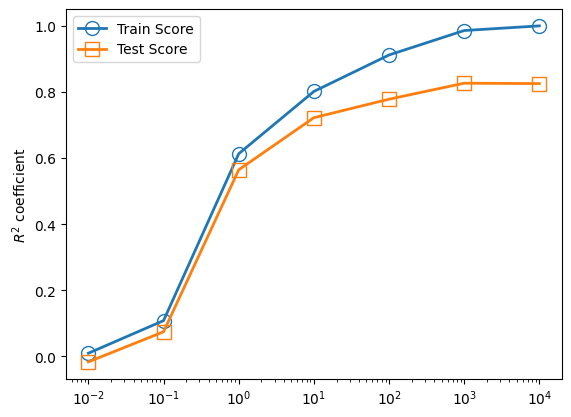
\includegraphics{../Figures/fig1-6.png}
    \caption{Comparing SVM regressors of different complexities on the
        Friedman-1 regression data set using $R^2$ as the evaluation metric. As with
        decision trees, highly complex models (corresponding to higher C values) appear
        to achieve fantastic fit on the training data, but they don’t actually generalize as
        well. This means that as C increases, so does the possibility of overfitting.}
\end{figure}

Every machine-learning algorithm, in fact, exhibits this behavior:
\begin{itemize}
    \item  Overly simple models tend to not fit the training data properly and tend to generalize poorly on future data; a model that is performing poorly on training
          and test data is underfitting.
    \item Overly complex models can achieve very low training errors but tend to generalize poorly on future data too; a model that is performing very well on training
          data, but poorly on test data is overfitting.
    \item The best models trade off between complexity and fit, sacrificing a little bit of
          each during training so that they can generalize most effectively when deployed.
\end{itemize}

\begin{tcolorbox}
    What we’ve informally discussed so far as the fit versus complexity tradeoff is more
    formally known as the bias-variance tradeoff. The bias of a model is the error arising
    from the effect of modeling assumptions (such as a preference for simpler models).
    The variance of a model is the error arising from sensitivity to small variations in the
    data set.

    Highly complex models (low bias) will overfit the data and be more sensitive to noise
    (high variance), while simpler models (high bias) will underfit the data and be less
    sensitive to noise (low variance). This tradeoff is inherent in every machine-learning
    algorithm. Ensemble methods seek to overcome this problem by combining several
    low-bias models to reduce their variance or combining several low-variance models to
    reduce their bias.
\end{tcolorbox}
\section{Our first ensemble}
We train a set of \textit{base estimators} (also known as \textit{base learners}) using diverse base-learning algorithms on the same data set. That is, \important{we count on the significant variations in each learning algorithm to produce a diverse set of base estimators.}

\section{Terminology and taxonomy for ensemble methods}
All ensembles are composed of individual machine-learning models called base models,
base learners, or base estimators (these terms are used interchangeably throughout the
book) and are trained using base machine-learning algorithms. Base models are often
described in terms of their complexity. Base models that are sufficiently complex (e.g.,
a deep decision tree) and have “good” prediction performance (e.g., accuracy over
80\% for a binary classification task) are typically known as strong learners or strong models.

In contrast, base models that are pretty simple (e.g., a shallow decision tree) and
achieve barely acceptable performance (e.g., accuracy around 51\% for a binary classi-
fication task) are known as weak learners or weak models. More formally, a weak learner
only has to do slightly better than random chance, or 50\% for a binary classification
task.

More broadly, ensemble methods can be classified into two types depending on
how they are trained: \textbf{parallel} and \textbf{sequential ensembles}.

Parallel ensemble methods, as the name suggests, train each component base
model \textit{independently} of the others, which means that they can be trained in parallel.
Parallel ensembles are often constructed out of strong learners and can further be categorized into the following:
\begin{itemize}
    \item \textbf{Homogeneous parallel ensembles}—All the base learners are of the same type (e.g.,
          all decision trees) and trained using the same base-learning algorithm. Several
          well-known ensemble methods, such as bagging, random forests, and extremely
          randomized trees (Extra Trees), are parallel ensemble methods.
    \item \textbf{Heterogeneous parallel ensembles}—The base learners are trained using different
          base-learning algorithms. Meta-learning by stacking is a well-known exemplar of
          this type of ensembling technique.
\end{itemize}

Sequential ensemble methods, unlike parallel ensemble methods, exploit the dependence of base learners. More specifically, during training, sequential ensembles train a new base learner in such \important{a manner that it minimizes mistakes made by the base learner trained in the previous step.} These methods construct ensembles sequentially in stages and often use weak learners as base models. They can also be further categorized into the following:

\begin{itemize}
    \item \textbf{Adaptive boosting ensembles}—Also called vanilla boosting, these ensembles train
          successive base learners by reweighting examples adaptively to fix mistakes in previous iterations. AdaBoost, the granddaddy of all the boosting methods, is
          an example of this type of ensemble method.
    \item \textbf{Gradient-boosting ensembles}—These ensembles extend and generalize the idea of
          adaptive boosting and aim to mimic gradient descent, which is often used
          under the hood to actually train machine-learning models. Some of the most
          powerful modern ensemble learning packages implement some form of gradient boosting (LightGBM), Newton boosting (XGBoost),
          or ordered boosting (CatBoost).
\end{itemize}

\begin{figure}
    \centering
    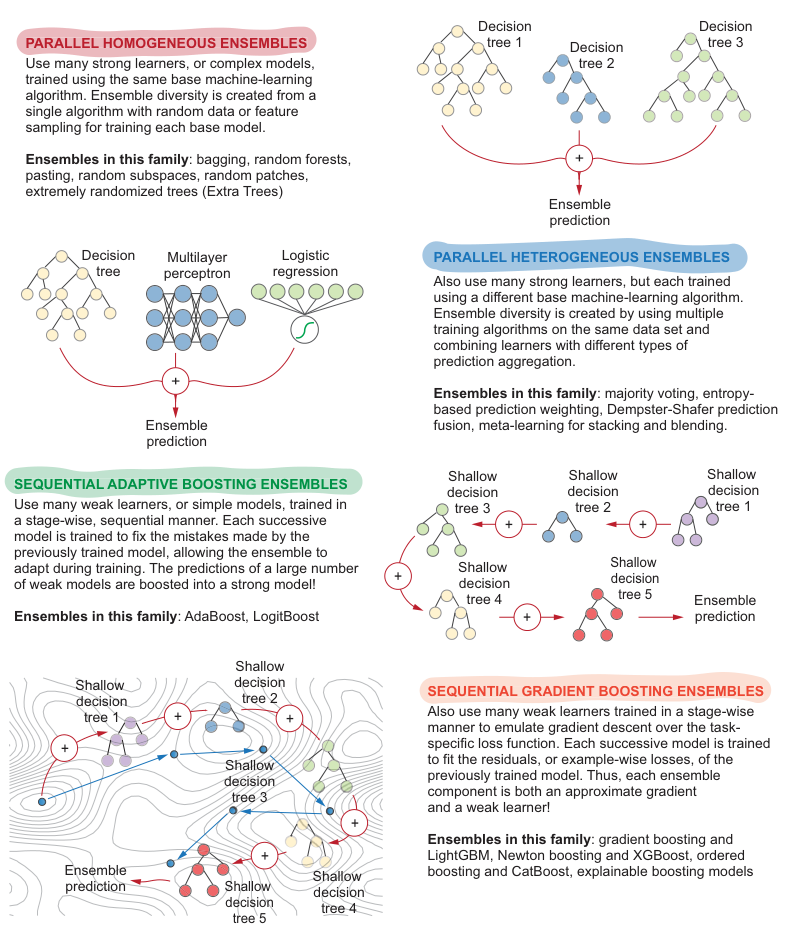
\includegraphics{../Figures/A taxonomy of ensemble methods.png}
    \caption{A taxonomy of ensemble methods}
\end{figure}

\section{Summary}

\begin{itemize}
    \item  Ensemble learning aims to improve predictive performance by training multiple models and combining them into a meta-estimator. The component models
          of an ensemble are called base estimators or base learners.
    \item  Ensemble methods use the power of “the wisdom of crowds,” which relies on
          the principle that the collective opinion of a group is more effective than any
          single individual in the group.
    \item  Ensemble methods are widely used in several application areas, including financial and business analytics, medicine and health care, cybersecurity, education,
          manufacturing, recommendation systems, entertainment, and many more.
    \item  Most machine-learning algorithms contend with a fit versus complexity (also
          called bias-variance) tradeoff, which affects their ability to generalize well to
          future data. Ensemble methods use multiple component models to overcome
          this tradeoff.
    \item  An effective ensemble requires two key ingredients: (1) ensemble diversity and
          (2) model aggregation for the final predictions.
\end{itemize}